% Additional file 1 --- supplementary information.
\documentclass[11pt]{article}
\usepackage[margin=1in]{geometry}
\usepackage{amsmath,amssymb,booktabs,graphicx,lmodern,longtable}
\usepackage[protrusion=true,expansion=false]{microtype}
\usepackage[colorlinks=true,linkcolor=blue,urlcolor=blue]{hyperref}
\usepackage{url}
\usepackage[labelfont=bf,font=small]{caption}
\usepackage{setspace}\setstretch{1.05}\setlength{\parskip}{0pt}
\graphicspath{{./}}
\newcommand{\hd}[1]{\medskip\par\noindent\textbf{#1}\par\nobreak\vspace{2pt}\noindent\ignorespaces}
\renewcommand{\thetable}{S\arabic{table}}
\renewcommand{\thefigure}{S\arabic{figure}}

\title{\vspace{-2em}\bfseries Additional file 1\\[4pt]
\large The encoder, not the bins: decomposing peak-level MS/MS gains}
\author{Xulin Pan \quad Chuanming Wang}
\date{}

\begin{document}
\maketitle

\noindent This file reports the per-arm and per-seed results behind every figure in
the main text, the full bootstrap distributions, and the peak-absorption analysis
broken down by acquisition condition. Every table here is also provided as a
machine-readable CSV in the repository under \texttt{results/}, and every number is
regenerated from saved run artefacts by \texttt{scripts/make\_supplementary.py} and
\texttt{scripts/make\_si\_figures.py}.

\section*{S1\quad Per-arm, per-seed metrics}

Table~\ref{tab:s1} gives every trained arm on both corpora. Twenty-seven training
runs: five arms $\times$ three seeds on the open corpus, four $\times$ three on the
single-library corpus. Parameter counts are
identical between M1R and M1 by construction, and the binned baseline M0 carries
$65\%$ more parameters than either.

\begin{table}[htbp]
\centering
\caption{Held-out metrics for every arm and seed. Macro AUPRC is the primary
metric; chance is $0.0085$ on the open corpus and $0.0093$ on the single-library
corpus. Machine-readable: \texttt{results/si\_table\_s1\_arm\_metrics.csv}.}
\label{tab:s1}
\small
\begin{tabular}{l l r r r r r r}
\toprule
corpus & arm & seed & parameters & best epoch & macro AUPRC & macro AUROC & Brier \\
\midrule
open & M0  & 2026 & 1,172,752 & 13 & 0.1433 & 0.8815 & 0.00531 \\
open & M0  & 7    & 1,172,752 & 14 & 0.1416 & 0.8793 & 0.00534 \\
open & M0  & 13   & 1,172,752 & 14 & 0.1406 & 0.8788 & 0.00535 \\
open & M1D & 2026 & 714,528   & 12 & 0.1616 & 0.8930 & 0.00522 \\
open & M1D & 7    & 714,528   & 13 & 0.1569 & 0.8915 & 0.00527 \\
open & M1D & 13   & 714,528   & 14 & 0.1585 & 0.8940 & 0.00524 \\
open & M1R & 2026 & 712,336   & 14 & 0.1591 & 0.8991 & 0.00525 \\
open & M1R & 7    & 712,336   & 13 & 0.1570 & 0.8980 & 0.00525 \\
open & M1R & 13   & 712,336   & 14 & 0.1541 & 0.8960 & 0.00526 \\
open & M1  & 2026 & 712,336   & 14 & 0.1731 & 0.9063 & 0.00513 \\
open & M1  & 7    & 712,336   & 13 & 0.1709 & 0.9063 & 0.00517 \\
open & M1  & 13   & 712,336   & 13 & 0.1687 & 0.9068 & 0.00514 \\
open & M2  & 2026 & 829,584   & 14 & 0.1899 & 0.9072 & 0.00512 \\
open & M2  & 7    & 829,584   & 14 & 0.1893 & 0.9052 & 0.00511 \\
open & M2  & 13   & 829,584   & 12 & 0.1871 & 0.9090 & 0.00512 \\
\midrule
single library & M0  & 2026 & 1,172,752 & 14 & 0.0631 & 0.8096 & 0.00689 \\
single library & M0  & 7    & 1,172,752 & 14 & 0.0621 & 0.8105 & 0.00688 \\
single library & M0  & 13   & 1,172,752 & 13 & 0.0608 & 0.8109 & 0.00688 \\
single library & M1R & 2026 & 712,336   & 13 & 0.0867 & 0.8457 & 0.00673 \\
single library & M1R & 7    & 712,336   & 14 & 0.0856 & 0.8474 & 0.00672 \\
single library & M1R & 13   & 712,336   & 14 & 0.0840 & 0.8470 & 0.00675 \\
single library & M1  & 2026 & 712,336   & 14 & 0.1119 & 0.8734 & 0.00654 \\
single library & M1  & 7    & 712,336   & 13 & 0.1085 & 0.8717 & 0.00656 \\
single library & M1  & 13   & 712,336   & 13 & 0.1162 & 0.8759 & 0.00652 \\
single library & M2  & 2026 & 829,584   & 13 & 0.1460 & 0.8861 & 0.00640 \\
single library & M2  & 7    & 829,584   & 13 & 0.1428 & 0.8824 & 0.00644 \\
single library & M2  & 13   & 829,584   & 14 & 0.1444 & 0.8837 & 0.00641 \\
\bottomrule
\end{tabular}
\end{table}

Every arm in both ladders is conditioned on the acquisition covariates (collision
energy, adduct, polarity, instrument). In earlier versions of this work M0 alone was
not: its encoder accepted the covariate vector and discarded it, so the binned
baseline was the only arm predicting without knowing how the spectrum had been
acquired. All six M0 rows above are refits under the corrected baseline and
supersede the figures reported previously; the main text states what the correction
cost the headline claim.

Conditioning was worth $+0.0288$ to M0 on the open corpus and $+0.0142$ on the
single-library corpus. That the gain roughly doubles with the corpus's acquisition
diversity --- $66$ instrument types and $112$ adducts against two and sixteen ---
is what one would expect if the covariates are doing the work we ascribe to them,
and we note it as a consistency check rather than a result.

\section*{S2\quad Per-seed effect sizes and ordering checks}

Each effect is the difference between two arms trained under the \emph{same} seed,
so the three values per row are matched rather than independent samples
(Table~\ref{tab:s2}). Where the main text claims an ordering between two effects, it
is checked within each seed; Table~\ref{tab:s3} reports those checks.

\begin{table}[htbp]
\centering
\caption{Effect sizes per seed, as differences in held-out macro AUPRC.}
\label{tab:s2}
\small
\begin{tabular}{l l r r r r r}
\toprule
corpus & effect & seed 2026 & seed 7 & seed 13 & mean & SD \\
\midrule
open & interface (M1D $-$ M0)   & $+0.0183$ & $+0.0153$ & $+0.0179$ & $+0.0172$ & 0.0016 \\
open & attention (M1R $-$ M1D)  & $-0.0025$ & $+0.0001$ & $-0.0045$ & $-0.0023$ & 0.0023 \\
open & encoder (M1R $-$ M0)     & $+0.0159$ & $+0.0154$ & $+0.0134$ & $+0.0149$ & 0.0013 \\
open & mass axis (M1 $-$ M1R)   & $+0.0140$ & $+0.0139$ & $+0.0147$ & $+0.0142$ & 0.0004 \\
open & aggregation (M2 $-$ M1)  & $+0.0168$ & $+0.0184$ & $+0.0184$ & $+0.0179$ & 0.0009 \\
\midrule
single library & encoder     & $+0.0236$ & $+0.0235$ & $+0.0232$ & $+0.0234$ & 0.0002 \\
single library & mass axis   & $+0.0252$ & $+0.0229$ & $+0.0322$ & $+0.0268$ & 0.0049 \\
single library & aggregation & $+0.0341$ & $+0.0343$ & $+0.0282$ & $+0.0322$ & 0.0035 \\
\bottomrule
\end{tabular}
\end{table}

\begin{table}[htbp]
\centering
\caption{Ordering checks. Each entry is the within-seed difference between two
effects; an ordering is reported in the main text only where it holds in all three
seeds.}
\label{tab:s3}
\small
\begin{tabular}{l l r r r r l}
\toprule
corpus & comparison & seed 2026 & seed 7 & seed 13 & mean & verdict \\
\midrule
open & encoder $-$ mass axis   & $+0.0019$ & $+0.0015$ & $-0.0012$ & $+0.0007$ & \textbf{reverses} \\
open & encoder $-$ aggregation & $-0.0009$ & $-0.0030$ & $-0.0049$ & $-0.0029$ & 3/3 consistent \\
open & mass axis $-$ aggregation & $-0.0028$ & $-0.0045$ & $-0.0037$ & $-0.0037$ & 3/3 consistent \\
\midrule
single library & encoder $-$ mass axis   & $-0.0016$ & $+0.0006$ & $-0.0090$ & $-0.0033$ & \textbf{reverses} \\
single library & encoder $-$ aggregation & $-0.0105$ & $-0.0108$ & $-0.0049$ & $-0.0087$ & 3/3 consistent \\
single library & mass axis $-$ aggregation & $-0.0089$ & $-0.0114$ & $+0.0041$ & $-0.0054$ & \textbf{reverses} \\
\bottomrule
\end{tabular}
\end{table}

Three things are worth reading off this table. The encoder-against-mass-axis row
reverses on both corpora independently, which is why the main text declines to order
those two anywhere. The encoder-against-aggregation row is consistent on both and
negative on both, which is why aggregation is the one ranking the paper does claim.
And the final row is why the main text ranks the mass axis against aggregation on
the open corpus and declines to on the single-library corpus.

\section*{S3\quad Bootstrap distributions}

Figure~\ref{fig:s1} shows the full distribution behind every interval reported in
the main text: $5{,}000$ resamples of the mean paired per-target difference, over
targets, after averaging each target's average precision across the three seeds.
Table~\ref{tab:s4} summarises them.

\begin{figure}[htbp]
\centering
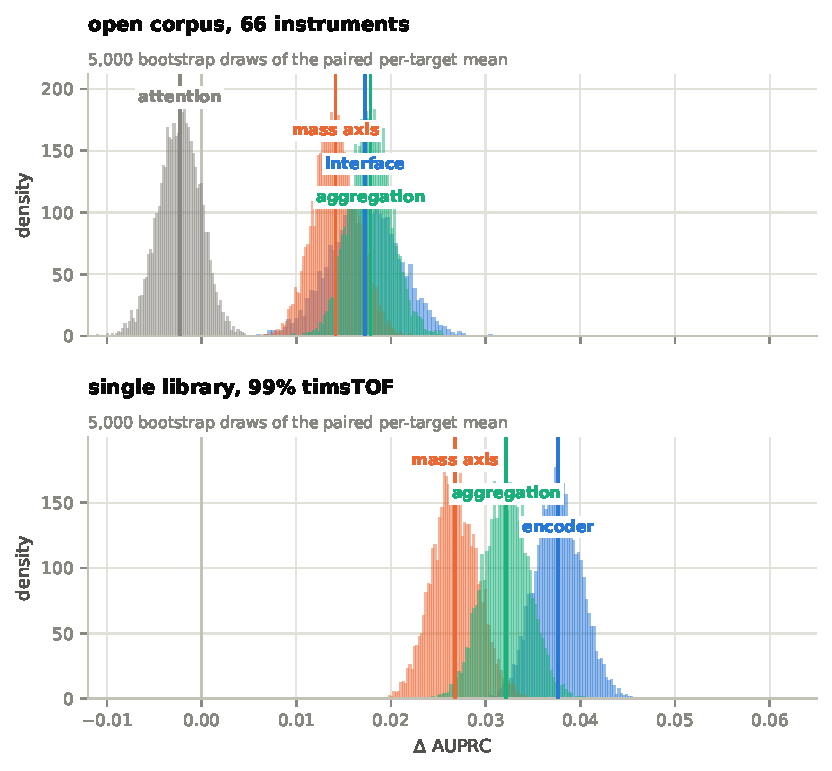
\includegraphics[width=0.66\linewidth]{figures/figS1_bootstrap_distributions.pdf}
\caption{Bootstrap distributions on each corpus. The open panel shows the encoder
split into its two components: the interface distribution sits far from the others
while the attention distribution is centred on zero. On the single-library corpus,
which has no attention arm, the composite encoder effect is shown instead. The
encoder and mass-axis distributions overlap heavily there, and the mass-axis and
aggregation ones likewise, which is the same fact Table~\ref{tab:s3} records as two
sign reversals; only the encoder and aggregation distributions separate.}
\label{fig:s1}
\end{figure}

\begin{table}[htbp]
\centering
\caption{Bootstrap summaries. Machine-readable draws:
\texttt{results/si\_table\_s3\_bootstrap\_draws.csv.gz}.}
\label{tab:s4}
\small
\begin{tabular}{l l r r r r}
\toprule
corpus & effect & mean & SD & 2.5\% & 97.5\% \\
\midrule
open & interface   & 0.01727 & 0.00360 & 0.01020 & 0.02419 \\
open & attention   & $-$0.00230 & 0.00221 & $-$0.00665 & 0.00196 \\
open & encoder     & 0.01498 & 0.00362 & 0.00798 & 0.02210 \\
open & mass axis   & 0.01415 & 0.00230 & 0.00969 & 0.01865 \\
open & aggregation & 0.01785 & 0.00222 & 0.01360 & 0.02233 \\
\midrule
single library & encoder     & 0.02344 & 0.00194 & 0.01972 & 0.02729 \\
single library & mass axis   & 0.02678 & 0.00243 & 0.02208 & 0.03168 \\
single library & aggregation & 0.03219 & 0.00243 & 0.02751 & 0.03696 \\
\bottomrule
\end{tabular}
\end{table}

\hd{What these intervals do and do not cover}
Each interval resamples targets, having first averaged average precision over the
three seeds. It therefore describes uncertainty from the finite set of targets, not
from initialisation. Seed variability is reported separately as the SD column of
Table~\ref{tab:s2}, and the two should be read together: on the single-library
corpus the mass-axis effect has a seed SD of $0.0049$, comparable to the width of
its bootstrap interval, which is the statistical form of the ordering failure in
Table~\ref{tab:s3}. A variance-components treatment with targets and seeds as
crossed random effects would fold both into one interval and we regard it as the
right analysis for a larger replicate count.

\hd{The attention arm}
M1D removes self-attention from every block while holding the mass axis, the peak
tokens and the acquisition conditioning fixed, so that $\mathrm{M1D}-\mathrm{M0}$
prices the interface and $\mathrm{M1R}-\mathrm{M1D}$ prices attention. Removing
attention frees $66{,}048$ weights per block; the feed-forward is widened to $548$
units in this arm alone so that the control is not also the smaller model
($714{,}528$ parameters against $712{,}336$). The attention effect is the only one
in this work whose interval includes zero, and it is also the only one positive in
fewer than three seeds of three.

\section*{S4\quad Per-target average precision}

\texttt{results/si\_table\_s2\_per\_target\_ap.csv} gives average precision for
every scored target, for every arm, both as the seed-averaged value used in the
paired analysis and per seed: $433$ targets on the open corpus and $477$ on the
single-library corpus, $910$ rows in total. All paired differences in the main text
are recoverable from this file by subtraction.

\section*{S5\quad Absorption by acquisition condition}

The main text reports that $23.6\%$ of the open corpus's held-out peaks fall into a
$0.5$~Da bin already occupied. Figure~\ref{fig:s2} breaks that down by adduct,
collision energy and instrument family.

\begin{figure}[htbp]
\centering
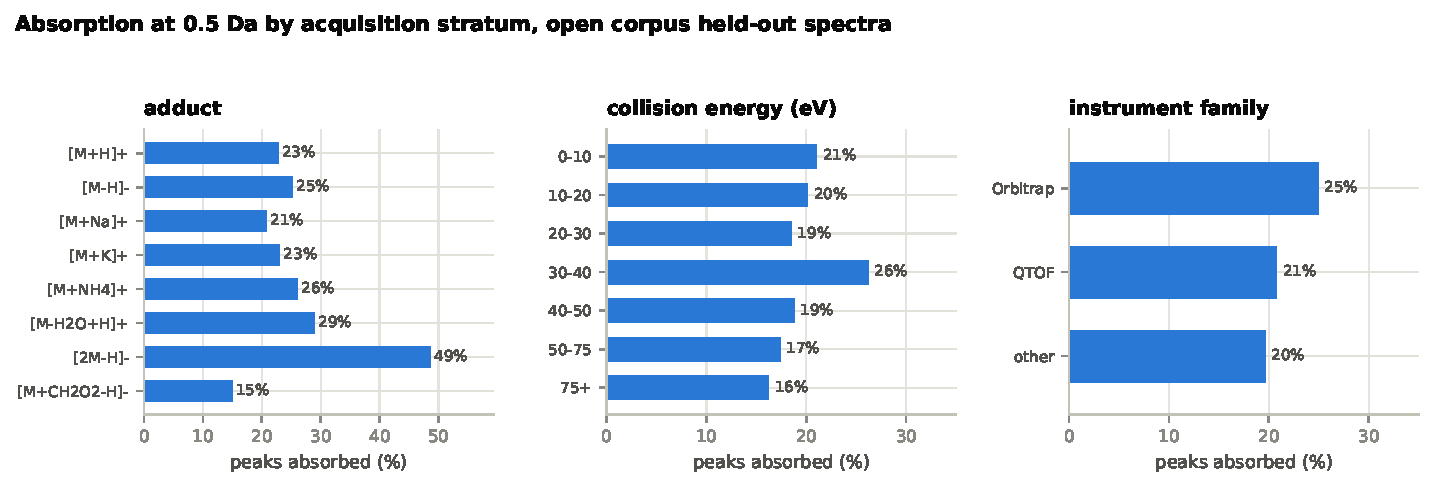
\includegraphics[width=\linewidth]{figures/figS2_absorption_strata.pdf}
\caption{Absorption at $0.5$~Da by acquisition stratum, over the open corpus's
held-out spectra. Strata with fewer than $20{,}000$ peaks are omitted.}
\label{fig:s2}
\end{figure}

Absorption tracks peak density rather than any chemical property of the adduct. The
highest rate among common adducts is $[2\mathrm{M}-\mathrm{H}]^-$ at $48.7\%$,
whose spectra are dimeric and correspondingly crowded; $[\mathrm{M}+\mathrm{H}]^+$,
which supplies $62\%$ of held-out spectra, sits at $22.8\%$. Across collision
energies the range is $16\%$ to $26\%$ with no monotone trend. Orbitrap spectra lose
$24.9\%$ against QTOF's $20.8\%$, again following density ($52.6$ against $47.2$
peaks per spectrum) rather than resolving power.

This is worth stating because it constrains the interpretation in the main text.
Binning costs more where peaks are dense, and density varies with acquisition
conditions that have nothing to do with how much mass precision the instrument
actually delivered.

\noindent Machine-readable, all under \texttt{results/}:
\begin{verbatim}
si_absorption_by_adduct.csv
si_absorption_by_collision_energy.csv
si_absorption_by_instrument_family.csv
\end{verbatim}

\section*{S6\quad Bin-width sweep}

Table~\ref{tab:s5} gives the sweep in full. Every arm uses the M1 encoder at an
identical parameter count; only the width of the mass grid changes. One run per
width, on the single-library corpus.

\begin{table}[htbp]
\centering
\caption{Bin-width sweep, single seed, single-library corpus.}
\label{tab:s5}
\small
\begin{tabular}{l r r r}
\toprule
bin width (Da) & peaks absorbed & macro AUPRC & share of the $0.5$~Da gap closed \\
\midrule
0.5            & 37.5\% & 0.0867 & 0\% \\
0.25           & 36.8\% & 0.0818 & $-19$\% \\
0.1            & 33.1\% & 0.0801 & $-26$\% \\
0.05           & 25.9\% & 0.0909 & 17\% \\
0.01           & 7.5\%  & 0.1030 & 65\% \\
full precision & 0.0\%  & 0.1119 & 100\% \\
\bottomrule
\end{tabular}
\end{table}

The absorption column here is computed over the competition test spectra, which are
denser than the corpus's own held-out spectra ($72.5$ against $58$ peaks per
spectrum); the corresponding held-out figures are $34.4\%$ at $0.5$~Da falling to
$6.5\%$ at $0.01$~Da, and those are the numbers the main text uses.

\section*{S7\quad Reproduction}

Software: Python 3.10, PyTorch 2.11.0+cu128, RDKit 2026.03.6, NumPy 2.4.4, pandas
2.3.3, pyarrow 24.0.0. Exact pins are in \texttt{requirements.txt}.

The full path from the corpus file to every number in this file is
\begin{verbatim}
python scripts/make_open_subset.py --root .
python -m dbf2 prepare --root . --dataset open
python -m dbf2 ablate  --root . --dataset open \
    --rungs M0 M1R M1 M2 --epochs 15
python -m dbf2 ablate  --root . --dataset open \
    --rungs M0 M1R M1 M2 --epochs 15 --seed 7
python -m dbf2 ablate  --root . --dataset open \
    --rungs M0 M1R M1 M2 --epochs 15 --seed 13
python scripts/make_supplementary.py
python scripts/make_si_figures.py
\end{verbatim}
with the same three commands minus \texttt{--dataset open} for the single-library
corpus, and
\begin{verbatim}
for w in 0.25 0.1 0.05 0.01; do
  python -m dbf2 train --root . --rung M1 \
      --quantise $w --tag W$w --epochs 15
done
\end{verbatim}
for the sweep. \texttt{python -m pytest src/dbf2/tests} runs $50$ unit tests, $14$
of which cover the rounding control, including that M1R and M1 have identical
parameter counts and that their configurations differ in exactly one field.

\hd{A note on what the subset builder reads}
\texttt{make\_open\_subset.py} selects the GNPS, MassBank and MoNA rows out of the
aggregated CASMI 2026 file. Those spectra are openly licensed at their sources, but
reproducing this work as written still requires that aggregated file. Fetching the
records from GNPS, MassBank and MoNA directly is recorded as an open item in the
repository. \texttt{docs/corpus\_composition.md} reports each source library's
contribution and states which parts are redistributable.

\end{document}
